\section{问题提出的背景}

\subsection{背景介绍}

浅地表地质目标的地球物理探测大多集中在几十厘米到几十米的范围,往往出于对工程设计的目的,对分辨率和定性定量解释有着更高的要求。但是由于探测对象本身拥有复杂的结构,以及地球物理场拥有的等效性,即不同的物理特征分布会得到相同的观测结果,以及观测系统在空间上覆盖的有限性和观测系统中包含的误差或是其他场源的影响,地球物理反演问题有着严重的非唯一性。电阻率法与地震走时成像作为浅地表勘探的两种重要方法,分别用于解决地下介质的电性差异与速度差异的问题。但是处于对探勘精度和问题的复杂性的考虑,单一的地球物理方法已经渐渐地无法满足目前的探测要求。例如电阻率法勘探,在浅地表中引起电性差异的原因主要是地层富水性的强弱,因电阻率勘探具有体积效应,在确定地层具有含水体的基础上无法确定含水量的大小。而含水量的确定是施工与设计最为关注的问题。另一方面,在对溶洞、空腔、煤层风氧化带的勘探时,此类带有容水空间的地质异常,在电阻率勘探中难以区分,因为空腔或裂隙中从充满空气到部分充水到完全充水,其在电阻率表现为从高电阻率到地层电阻率背景值再到低电阻率形态变化。

在地震走时勘探中, 速度不均匀体在射线路径上分布,在同时改变不均匀体的大小和速度值的情况下可以使接收点上获得相同的走时分布,在高速或低速异常周围容易形成拖尾异常。 针对地球物理方法多解性以及单一方法无法解决浅地表工程地质问题的情况,多种岩石属性数据联合反演解释成为一种有效途径。

\subsubsection{前人研究}

前人对基于岩石物理关系的联合反演也做了较多的研究,例如Colombo等建立了密度、电阻率与速度的经验关系,并通过重、电、震数据联合反演圈定了隐伏盐丘;De Stefano等利用Gardner公式建立了地层密度与地震纵波速度的关系式,开展重力与地震旅行时数据联合反演,并通过理论模 型 测 试 表 明 联 合 反 演 能 提 高 成 像精度。

Zhdanov等研究一种不需要Gramian约束的地球物理数据联合反演,此种方法不需要定义模型之间的关系函数。而近年来聚类的思想被引入联合反演中,研究者发现此类方法可以解决传统的统计方法难以将多组岩石物理关系应用于特定区域的难题。除了利用直流电法-地震数据进行联合反演外,Cater-Mcauslan等大量研究者也提出了基于重力-地震数据的联合反演。陈晓等提出基于宽范围岩石物性约束的大地电磁与地震联合反演,该类方法可降低由于先验岩石物理关系不够精确带来的影响。胡祖志等利用已知的测井、地震剖面等先验信息进行约束建模,并基于井—震约束的MT和重力数据实现了人工鱼群联合反演。相鹏等提出一种变密度—速度关系的重力与地震同步联合反演方法。杨博等提出了一 种基于聚类和多元地质统计学的电-震联合建模约束反演方法。

\subsection{本研究的意义和目的}

单一地球物理勘探方法不可避免地具有片面性和局限性,因此本研究可以对提 高对目标地质体的识别能力,利用聚类方法对电法和地震数据进行联合建模反演,提高对异常体边界的刻画能力,同时改善电法和地震方法单独反演结果,一定程度上提高反演计算速度。本研究在联合反演、物性参数关系联合反演的基础上进行算法改进和策略优化,在多个实例中尝试解决联合反演的相关问题。

开发一种可以有效利用多模态岩石物理信息的联合反演策略具有重要意义,它可以有效地解决岩石物理信息的非唯一性问题。以图 1 中的岩石物理数据为例(即 Moorkamp 等人,2013 年的图 4)。 黑点显示了穿透海洋盐丘的钻孔的电阻率和地震速度测量值。 尽管由于测量噪声和钻孔附近的局部不均匀性造成了分散,图 1 中测得的电阻率和速度值(即黑点)的交会图显示了两个主要的聚类特征,一个被蓝色圆圈包围并对应于 盐和另一个表现出准二次趋势并代表背景沉积物。 图 1 中物性分布的双峰性质反映了该地区的真实地质情况。 但与此同时,也使得在联合反演中使用这些有价值的信息变得困难,因为当存在多个岩石物理关系时,几乎不可能事先正确指定这些岩石物理关系的空间适用性。 如果我们不能对适当的区域应用适当的岩石物理约束,如图 1 所示的先验岩石物理信息,尽管其本身非常有价值,但要么无效,要么甚至对反演产生负面影响。

\begin{figure}
    \centering
    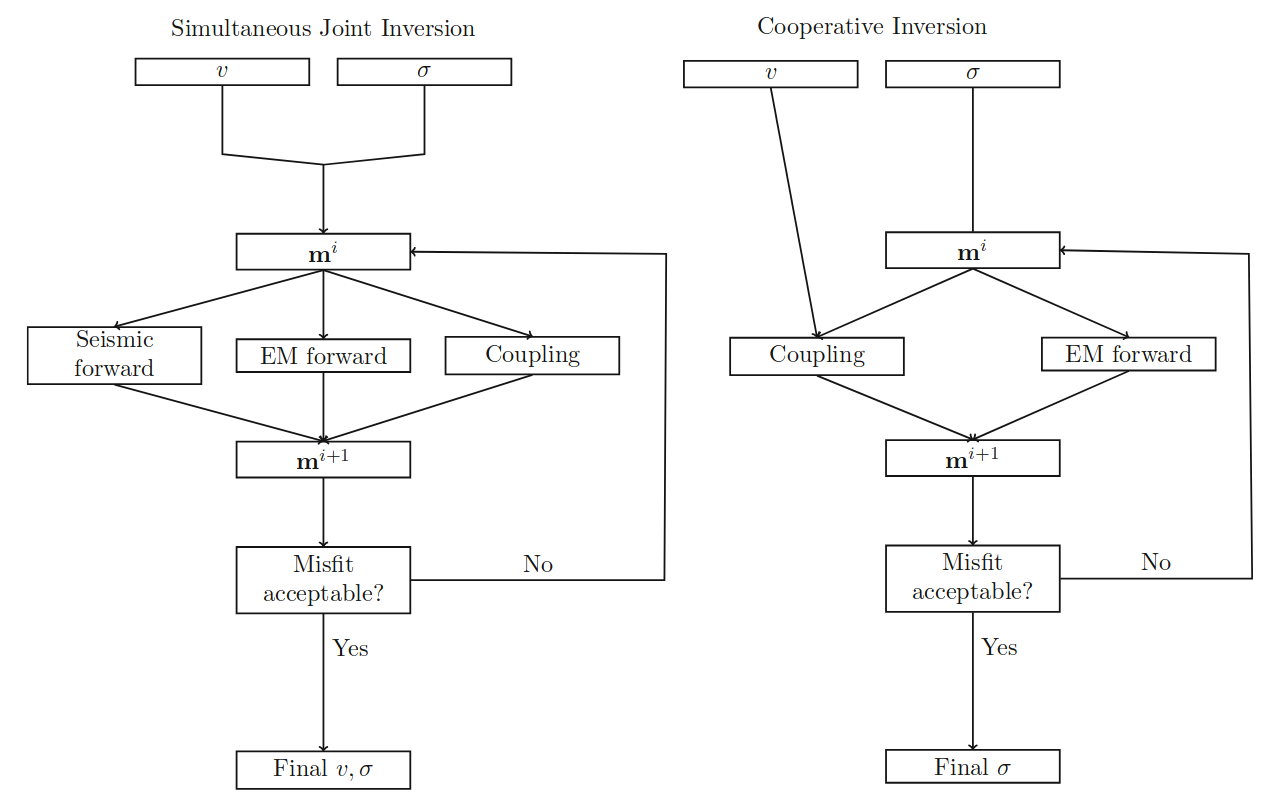
\includegraphics[width=0.9\textwidth]{trans/trans_1.png}
    \caption[]{联合反演算法(左)和协同反演算法(右)的简化流程图(Moorkamp等, 2016 b)。两种方法之间的主要区 别在于,对于协同反演,进入耦合约束的一个量(此处地震速度 v)在整个反演过程中不会发生变化,而所有量都在联合反演中进行调整} \label{ktbg1}
\end{figure}